Before performing the actual learning and prediction tasks, this chapter explores the data
in order to understand the statistics of the different features.

\subsection{Features}

After pre processing the data the data set to be explorted is describe in the following table:

\begin{table}[ht!]
\begin{center}
\begin{tabular}{llllrr}
\toprule
Field &  Description & Type &\\
\midrule
     Previous Dialog Act & dialog act before the current one  & categorical\\
     Dialog Act & current dialog act & categorical \\
     Length & length of the current dialog act in seconds & numeric \\
     Relative Turn Length(in seconds) (RTL)  & The length of the current dialog act in seconds & numeric \\
     Relative Time Control(in seconds) (RTC) & length of the current turn in words & numeric \\
     Turn Change & 1 if there was a turn change after this dialog act & binary \\
\bottomrule
\end{tabular}
\end{center}
\caption{Data Fields}
\end{table}


\subsection{Dialog Acts}

Figure \ref{dactsizefig} shows the count for each dialog act. We can observe that the majority of dialog acts are statements, backchannels and opinions. This is true to the nature of the switchboard corpus
which consists mainly of casual conversations. 

 \begin{figure}[ht!]
 \centering
 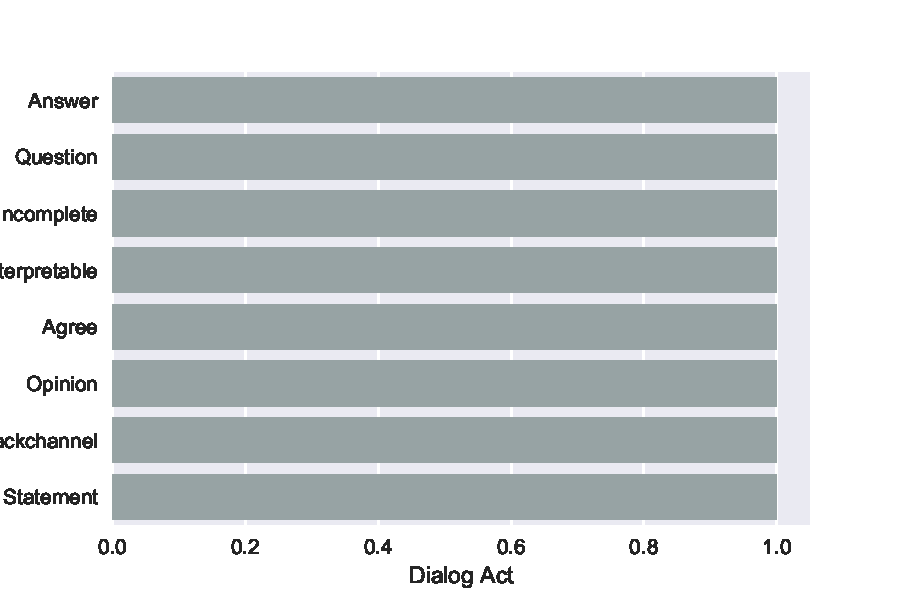
\includegraphics[width=0.5\textwidth]{../scikitlearn/figures/countplot_da_name_count.pdf}
 \caption{Dialog act size\label{overflow}}
 \label{dactsizefig}
 \end{figure}

Figure \ref{dactssecsbyname} shows an histogram of the length in seconds for each dialog act. It is evident that the distribution is left tilted.

 \begin{figure}[ht!]
 \centering
 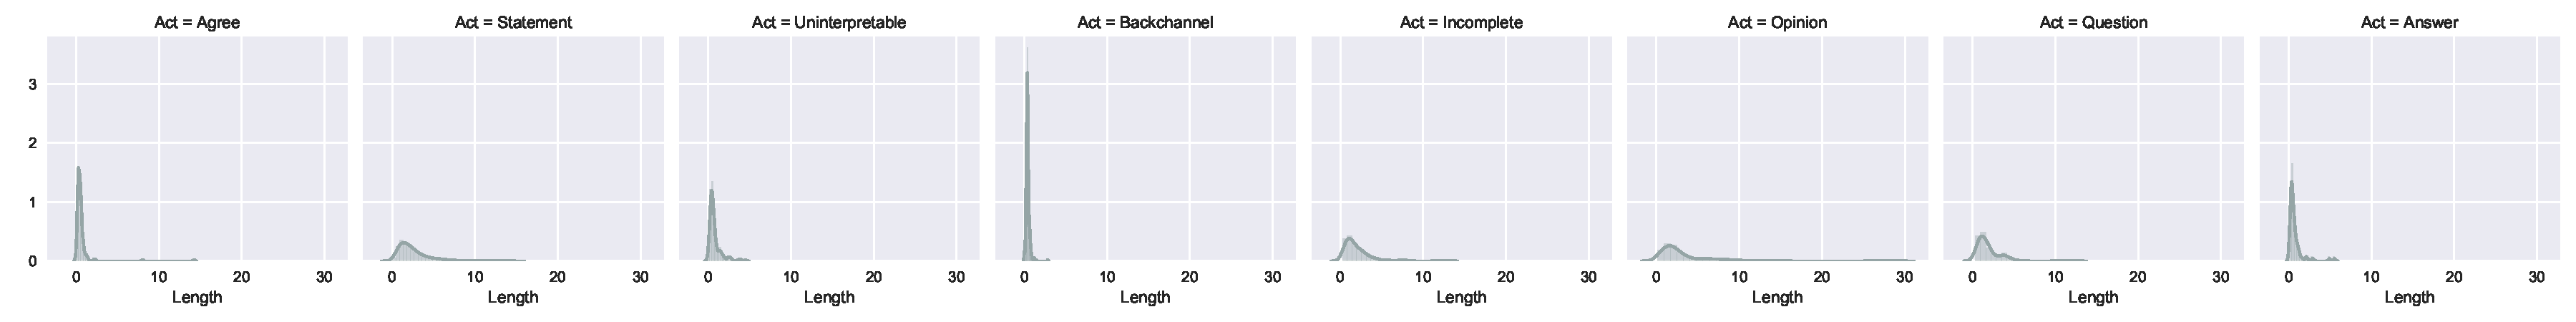
\includegraphics[width=\textwidth]{../scikitlearn/figures/grid_secs_by_da_name.pdf}
 \caption{Dialog act length in words \label{overflow}}
 \label{dactssecsbyname}
  \end{figure}
 
 Figure \ref{l3} shows the and histogram for each dialog act length conditioned on the occuruce of a turn change. We can observe that the length distribution is the same, however when a turn change occur, some
 dialog acts tends to be longer than regular. 
 
\begin{figure}[ht!]
 \centering
 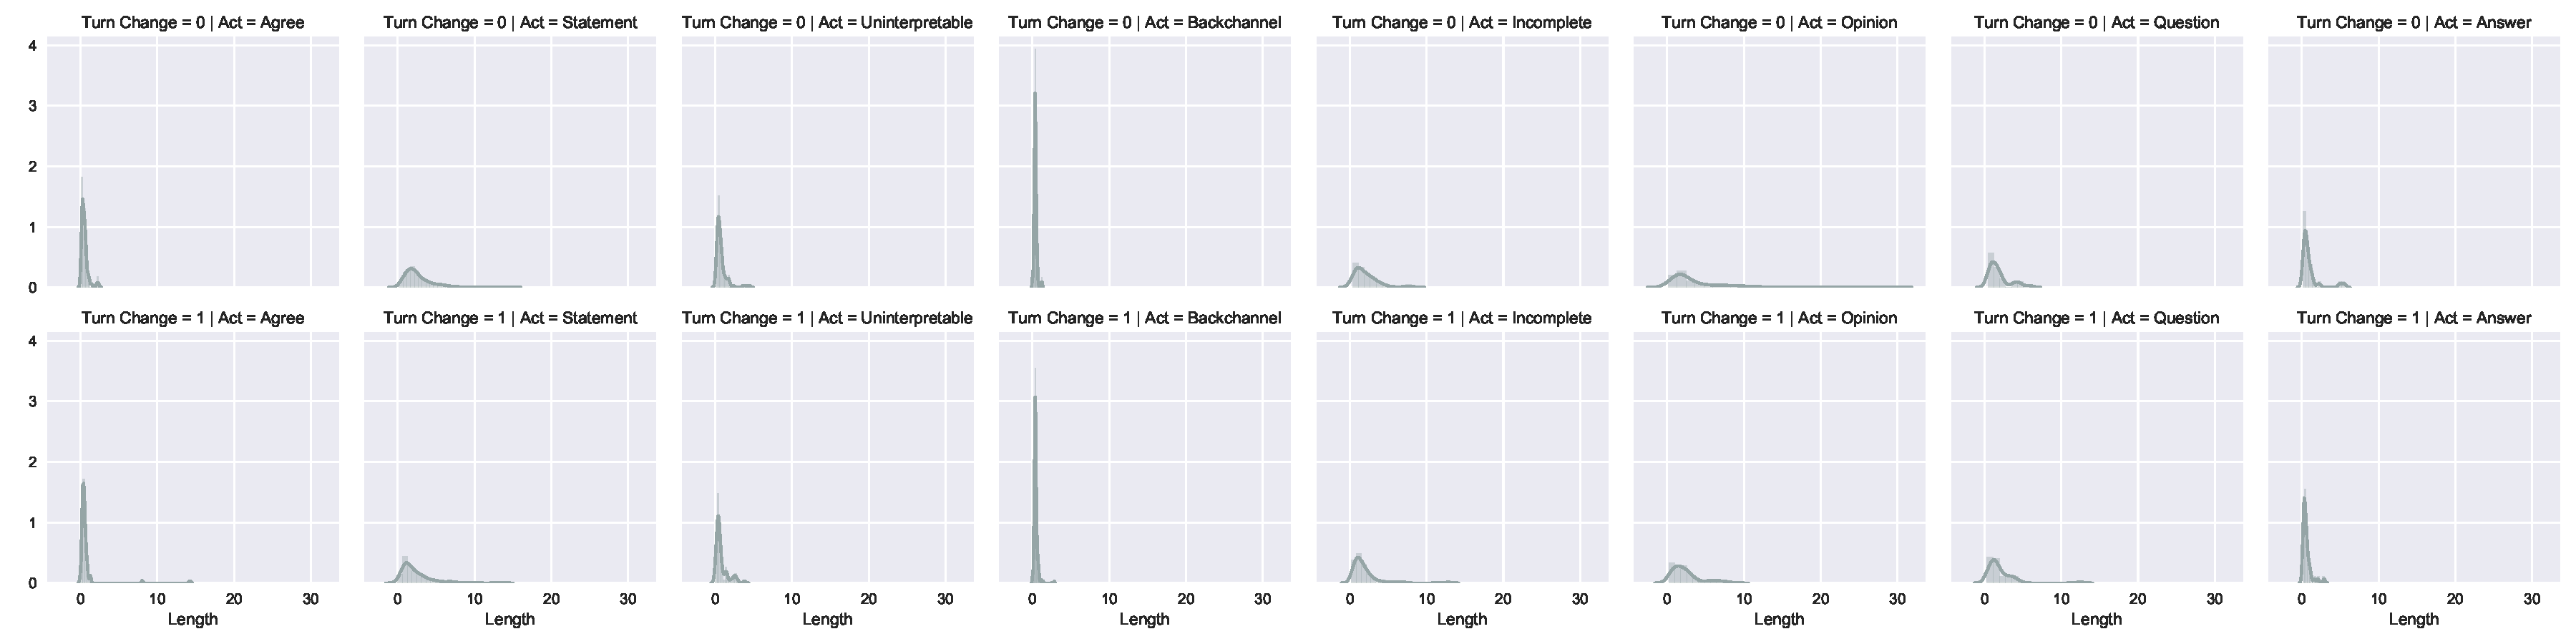
\includegraphics[width=\textwidth]{../scikitlearn/figures/grid_secs_by_da_name_by_tchange.pdf}
 \caption{Dialog act length in words conditioned on turn change\label{overflow}}
 \label{l3}
 \end{figure}
 
In figure \ref{l4} , we measure the probability that a dialog act will lead to turn change. We can observe that the majority of back channels and question will lead to a turn change.  

\begin{figure}[ht!]
\centering
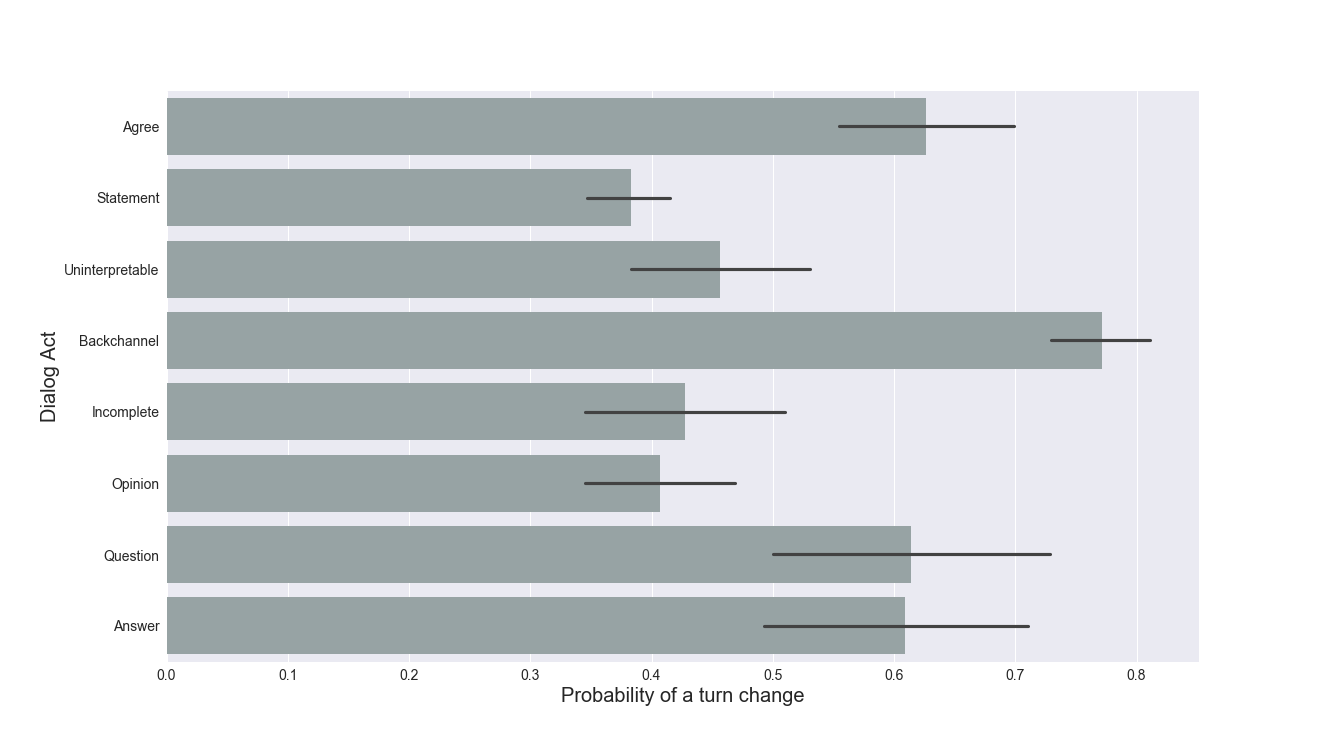
\includegraphics[width=0.5\textwidth]{../scikitlearn/figures/barplot_da_prob_to_tchange.png}
\caption{Dialog act probability of turn change\label{overflow}}
\label{l4}
\end{figure}


\subsection{Relative Turn Length}

Figure \ref{l5} shows the distribution of the relative turn length for each dialog act. We can observe
that 

\begin{figure}[ht!]
\centering
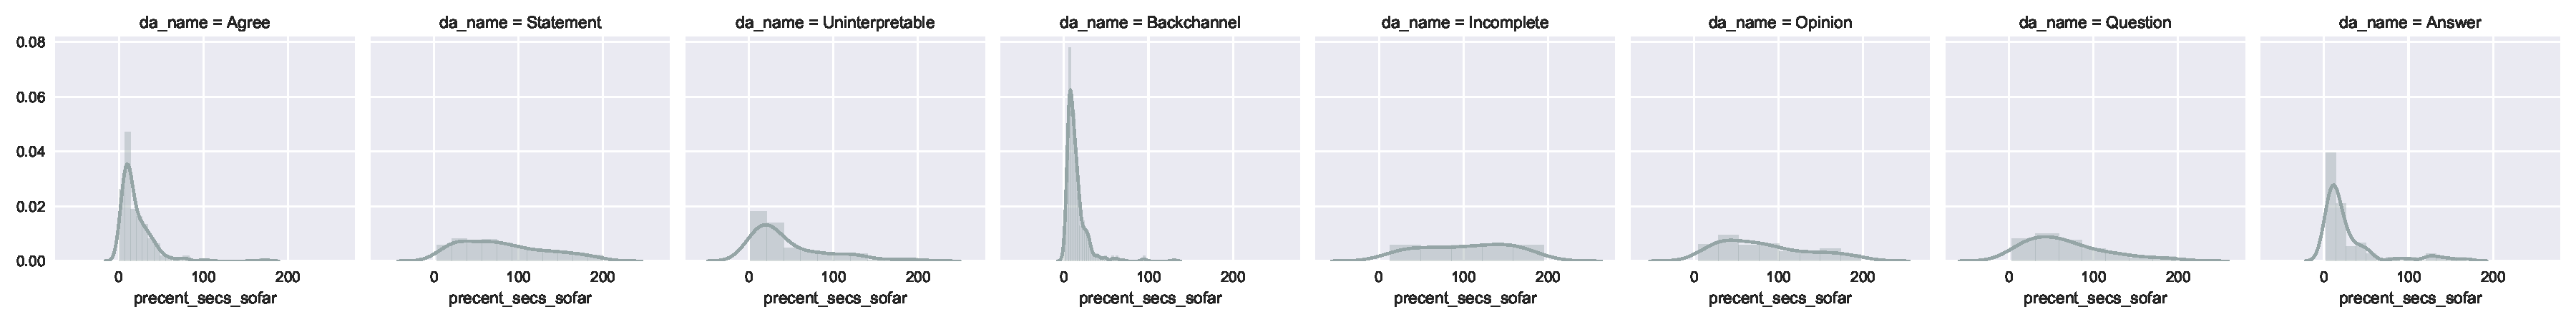
\includegraphics[width=\textwidth]{../scikitlearn/figures/grid_precent_secs_sofar_by_da_name.pdf}
\caption{Relative turn length for each dialog act\label{overflow}}
\label{l5}
\end{figure}
 

\subsection{Relative Floor Control}

Figure \ref{l6} shows distribution of floor control or each dialog act conditioned on a turn change. We can observe that regardless of the dialog act, most distributions are normal with mean of 50\%

\begin{figure}[ht!]
\centering
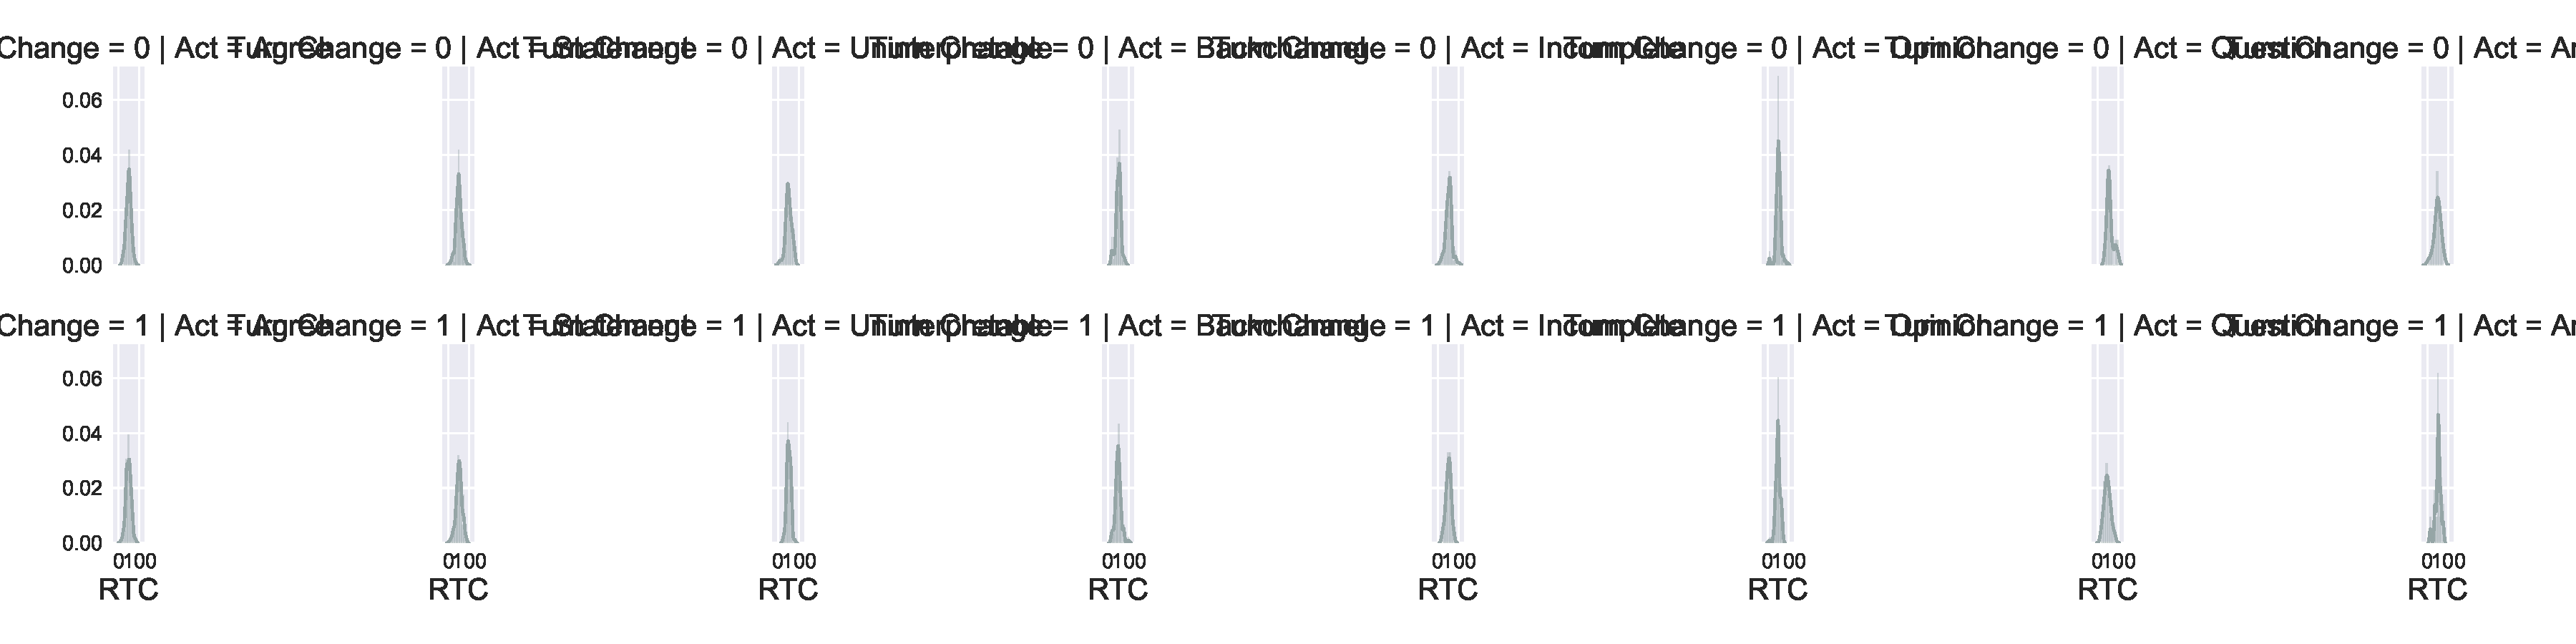
\includegraphics[width=\textwidth]{../scikitlearn/figures/grid_timecontrol_by_da_name_by_tchange.pdf}
\caption{Relative flow control conditioned on turn change\label{overflow}}
\label{l6}
\end{figure}


